\documentclass[a4paper]{article}
\usepackage[newfloat]{minted}
\usepackage{graphicx}
\usepackage{caption}
\usepackage{amsmath}
\usepackage{amsfonts}
\usepackage[a4paper,left=3cm,right=2cm,top=2.5cm,bottom=2.5cm]{geometry}
\usepackage[colorlinks=true, urlcolor=blue, pdfborder={0 0 0}]{hyperref}
\usepackage{subcaption}
\newenvironment{code}{\captionsetup{type=listing}}{}
\SetupFloatingEnvironment{listing}{name=Code}

\title{RL Homework 4}
\author{Ananth Mahadevan}
\begin{document}
\maketitle
\clearpage


\section*{Question 1}
I think it is not possible to learn the Q-values for Cartpole from just providing linear features to a linear regression. This is because the Cartpole environment might not have linear dynamics. This then means that the state features are not enough for the Q-values to converge. This is because the linear regressor with state features has too little expressive power to capture the non-linear dynamics of the Cartpole system. This might be inherent as the stable state in the physical system might be to optimize for energy of the pole. This then means we have a quadratic dependence on the velocity of the cart and the angular speed. Hence the linear state features might be insufficient to learn.

\begin{figure}[h!]
    \centering
    \begin{subfigure}[b]{0.49\textwidth}
        \centering
        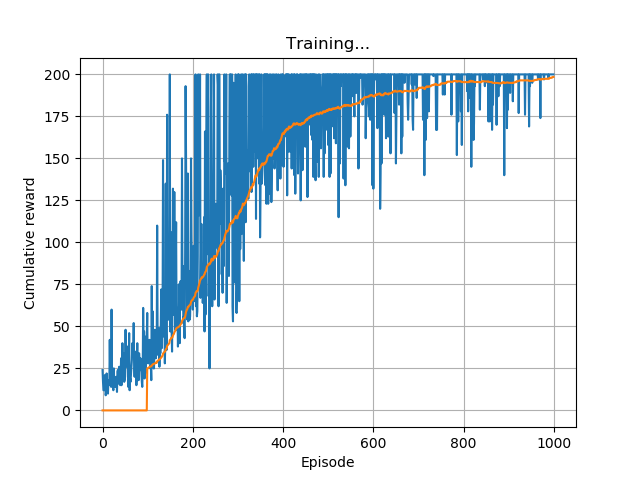
\includegraphics[width=\textwidth]{training_rbf.png}
        \caption{RBF Features}
        \label{fig-rbf-single}
    \end{subfigure}
    \begin{subfigure}[b]{0.49\textwidth}
        \centering
        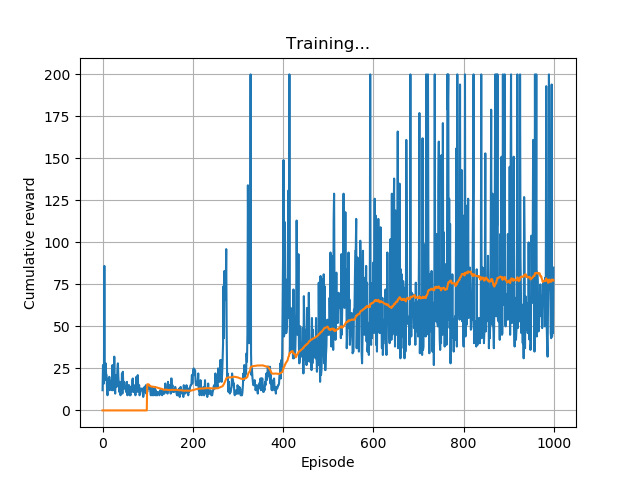
\includegraphics[width=\textwidth]{training_handcrafted.png}
        \caption{Handcrafted Features}
        \label{fig-handcrafted-single}
    \end{subfigure}
    \caption{Training Plots for different methods}  
    \label{fig-single-update}
\end{figure}
\section*{Task 2}
\begin{figure}[h!]
    \centering
    \begin{subfigure}[b]{0.49\textwidth}
        \centering
        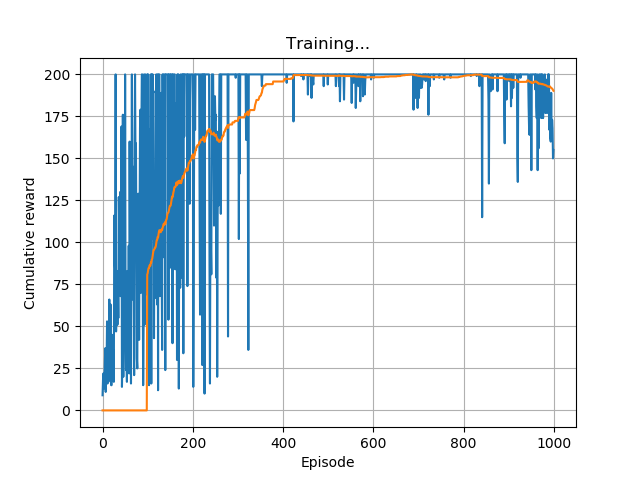
\includegraphics[width=\textwidth]{training_rbf_experience_replay.png}
        \caption{RBF Features}
        \label{fig-rbf-minibatch}
    \end{subfigure}
    \begin{subfigure}[b]{0.49\textwidth}
        \centering
        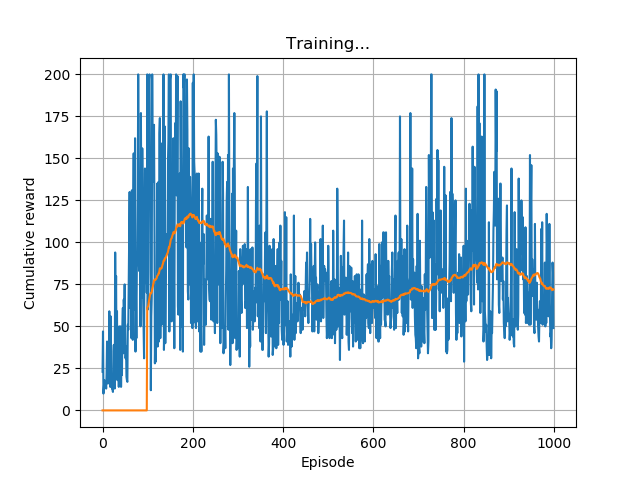
\includegraphics[width=\textwidth]{training_handcrafted_experience_replay.png}
        \caption{Handcrafted Features}
        \label{fig-handcrafted-minibatch}
    \end{subfigure}
    \caption{Minibatch Update for different methods}
    \label{fig-minibatch-update}
\end{figure}
\subsection*{Question 2.1}
The RBF features with experience replay from the Figure is the most sample efficient method compared to the other methods. This method learn much faster and by around 200 episodes there is already an optimal policy. The reason that this method is most sample efficient is because it has experience replay, this allows the model to get more efficient estimate of the gradient using more samples in the minibatch. This allows the update to converge to an optimal policy using much fewer samples. The RBF features are also make the linear model more expressive.  
\subsection*{Question 2.2}
The handcrafted features are inefficient as the features are not expressive enough for the model. This means that the state and its absolute value are not of good quality. There are also too few features compared to the RBF features (8 vs 230). Smaller number of features usually train faster but is tradeoff for the quality. Handcrafted features can be made better by doing some feature selection on the model. Maybe we can gather more non-linear features like the square of the state or gather more based on domain experience, then we can do feature engineering/selection to choose the most important/useful features.
\subsection*{Question 2.3}
Grid based methods are not very sample efficient especially when compared to the function approximation methods. The main reason is that for grid based methods we need to sample states to specifically update a particular grid value, if we don't have many samples then a lot of the grid values end up not getting updated. This then leads to the policy not converging to an optimal value. The reason that function approximation is better and more sample efficient is that an update for a particular state also updates the whole function space, hence other states are also updated to a certain amount. This then means that we don't need to have samples to update every state but enough so that the whole function is converging to optimal values.
\subsection*{Question 2.4}
Hyperparameter such as the number of features or the $\epsilon$-greedy exploration value for GLIE might impact the efficiency. The number of features means that the function approximation will be more expressive for the linear methods. More features might also make the methods slower per iteration. The value of $a$ for GLIE will also affect the rate of exploration for the model and that in turn affects the efficient. Other hyperparameter might be the learning rate of the linear model, the optimizer that is used.
\section*{Question 3}
\begin{figure}[h!]
    \centering
    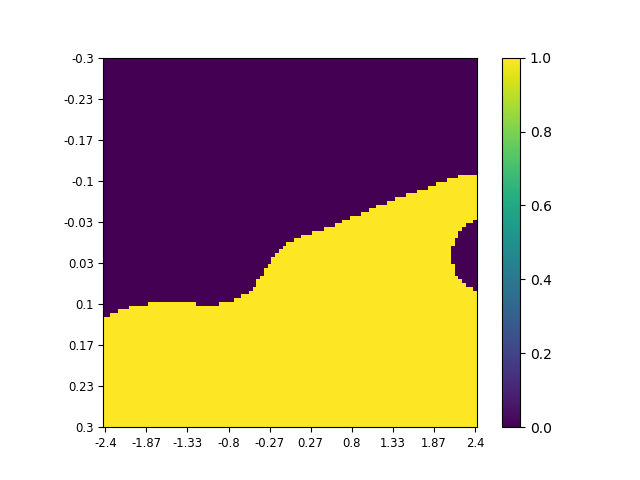
\includegraphics[width=0.5\textwidth]{policy.png}
    \caption{2D Policy Plot (x-axis is $x$ and y axis is $\theta$) with $\dot{x}=\dot{\theta}=0$ for the RBF features method}
    \label{fig-policy}
\end{figure}

\begin{figure}[h!]
    \centering
    \begin{subfigure}[b]{0.49\textwidth}
        \centering
        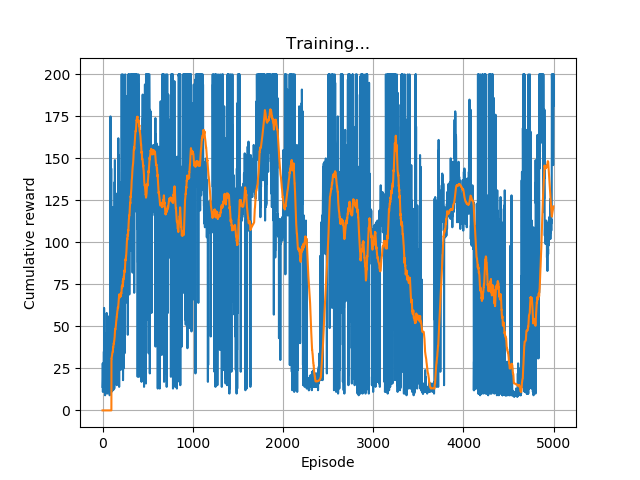
\includegraphics[width=\textwidth]{training_CartPole-v0.png}
        \caption{Cartpole Environment}
        \label{fig-cartpole-DQN}
    \end{subfigure}
    \begin{subfigure}[b]{0.49\textwidth}
        \centering
        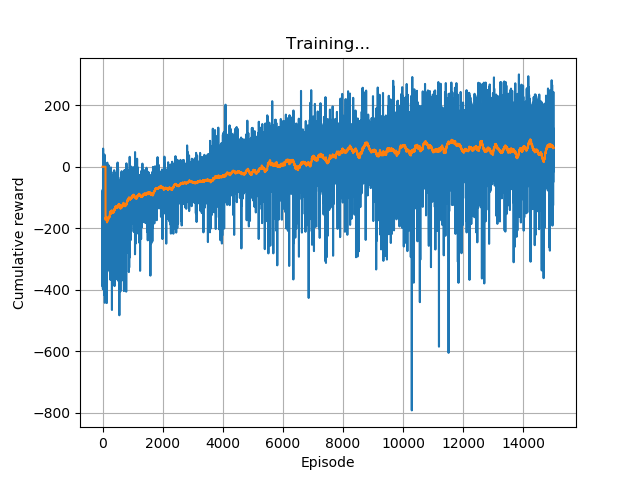
\includegraphics[width=\textwidth]{training_LunarLander-v2.png}
        \caption{Lunar Lander Environment}
        \label{fig-lunar-DQN}
    \end{subfigure}
    \caption{DQN training plots for different environments}
    \label{fig-DQN}
\end{figure}
\subsection*{Question 3.1}
Q learning cannot be directly used in environments with continuous action spaces. The expected target result for the Q-value must be changed/extended to work well in situations with continuous action spaces. The easiest way to directly implement Q-learning would be to discretize the action space and then utilize Q-learning as we would. The issue with this method would be that the variance might be too high and convergence might not be guranteed. 
\subsection*{Question 3.2}
In Q-learning the update step consists of computing the target Q-value for the particular sample from the environment as 
\[ Q(s,a) \leftarrow Q(s,a) + \alpha\left[ R_{t+1} +\gamma\max_{a'} Q(s',a') - Q(s,a) \right]\] 
The biggest issue in this is finding the maximal next state action value given the current state, action and reward that is accrued. This will be impossible in environments when the action space is continuous and possibly infinite.

The fix to this would be to then sample a possible action to estimate the performance of the policy. This is the idea behind \textit{action-critic} methods that do especially that, sample an action from the current policy and then compute the target with the discounted reward and the probability of taking the actions. 
\end{document}